\section{PROJE'NİN İŞLEYİŞİ}
\subsection{Arayüz Kısmı }
Bu projede arayüz kısmı için belirtilen işleyiş aşağıda açıklanmaktadır. Uygun bir template bulunmuş ve projeye uygun hale getirilmiştir. Gereksiz kısımlar temizlenerek sağ menü bölümünde Dashboard, görevler (Ping, Theharvester), sistem logları ve Profil bölümleri oluşturulmuştur.\\
Projeyi ilk açtığınızda, kullanıcı login sayfasıyla karşılaşacaksınız. Kimlik bilgilerinizi girdikten sonra doğrulama yapıp diğer sayfalara erişebileceksiniz. Giriş yaptıktan sonra karşılaşacağınız ilk sayfa Kontrol Paneli olacaktır. Kontrol panelinde gerçekleştirilebilecek işlemler açıklanacaktır.\\
Sağ kısımda menü bulunmaktadır. Buradan istediğiniz zaman görevler bölümünden görev oluşturabilir ve önceden oluşturulan görevle ilgili işlemleri görebilirsiniz. Bir Ping görevi oluşturulduğunda, bu konteynırların çıktıları, kayıp yüzdesi, pingin maksimum geri dönüş süresi, minimum geri dönüş süresi ve ortalama milisaniye geri dönüş süresi gibi bilgilere erişebilirsiniz. Ayrıca sağ menüde sistem log kayıtlarını görüntüleyebilirsiniz. Log kayıtlarının altında kullanıcının hangi görevi ne zaman çalıştırdığı, görevin tamamlanma süresi, başarılı veya başarısız olma durumu ile oturum açma ve kapatma bilgileri kolaylıkla görüntülenebilir.\\
Hesabım bölümü, profili ile ilgili düzenlemeler yapmayı sağlar. Bu bölümde profil bilgilerini güncelleyebilir, şifreniyi değiştirebilir, iletişim tercihlerini yönetebilir ve gizlilik ayarlarını düzenlenebilir. Bu şekilde, profili yönetebilir ve hesap istediğimiz  şekilde kişiselleştirebilir hale getirildi.
%arayüz fotoğrafları eklenecek 
\subsection{Arka paln işleyişi}

%ibrahim bu kısımda özet yazacak detaylandırılacak
 \subsection {Veritabanı kısmı İçin }
 MySQL veritabanı kullanılarak bir proje için optimize edilmiş bir veritabanı şeması oluşturuldu. Bu şema, "users" (kullanıcılar), "ping" (ping kayıtları) ve "pingcontainers" (ping konteynerleri) adında üç tabloyu içermektedir. Bu düzenleme, veritabanının performansını artırmak ve veri bütünlüğünü sağlamak amacıyla yapılmıştır.\\
"users" tablosu, kullanıcıların temel bilgilerini içerir ve her kullanıcıya birincil anahtar (ID) ile benzersiz bir kimlik atar. Ayrıca kullanıcı adı, e-posta adresi ve diğer ilgili bilgiler gibi sütunlar da içerir.\\
"pingcontainers" tablosu, kullanıcıların oluşturabileceği ping konteynerlerini temsil eder. Her konteyner birincil anahtar ile tanımlanır ve kullanıcıya ait olacak şekilde kullanıcı kimliği (user ID) ile ilişkilendirilir. Bu tablo, kullanıcının birden fazla konteyner oluşturabilmesine olanak sağlar.\\
"ping" tablosu, gerçekleşen ping olaylarını kaydetmek için kullanılır. Her ping kaydı, birincil anahtar ile tanımlanır ve bir konteynere (container ID) ve kullanıcıya (user ID) bağlanır. Bu ilişki, her ping kaydının hangi kullanıcı ve konteyner tarafından oluşturulduğunu gösterir.\\
Bu veritabanı şeması, kullanıcıların birden fazla konteyner ve görev oluşturabilmesini sağlar. Ayrıca, her görevin bir kullanıcı tarafından oluşturulduğu ilişkisi sayesinde veri bütünlüğünü korur.\\
Bu düzenleme, veritabanının daha etkili bir şekilde veri saklamasını ve verilere hızlı erişim sağlamasını amaçlamaktadır. Ayrıca, veri bütünlüğünü korumak için gereken ilişkileri de sağlamaktadır.\\
 \begin{figure}[htbp]
    \centering
    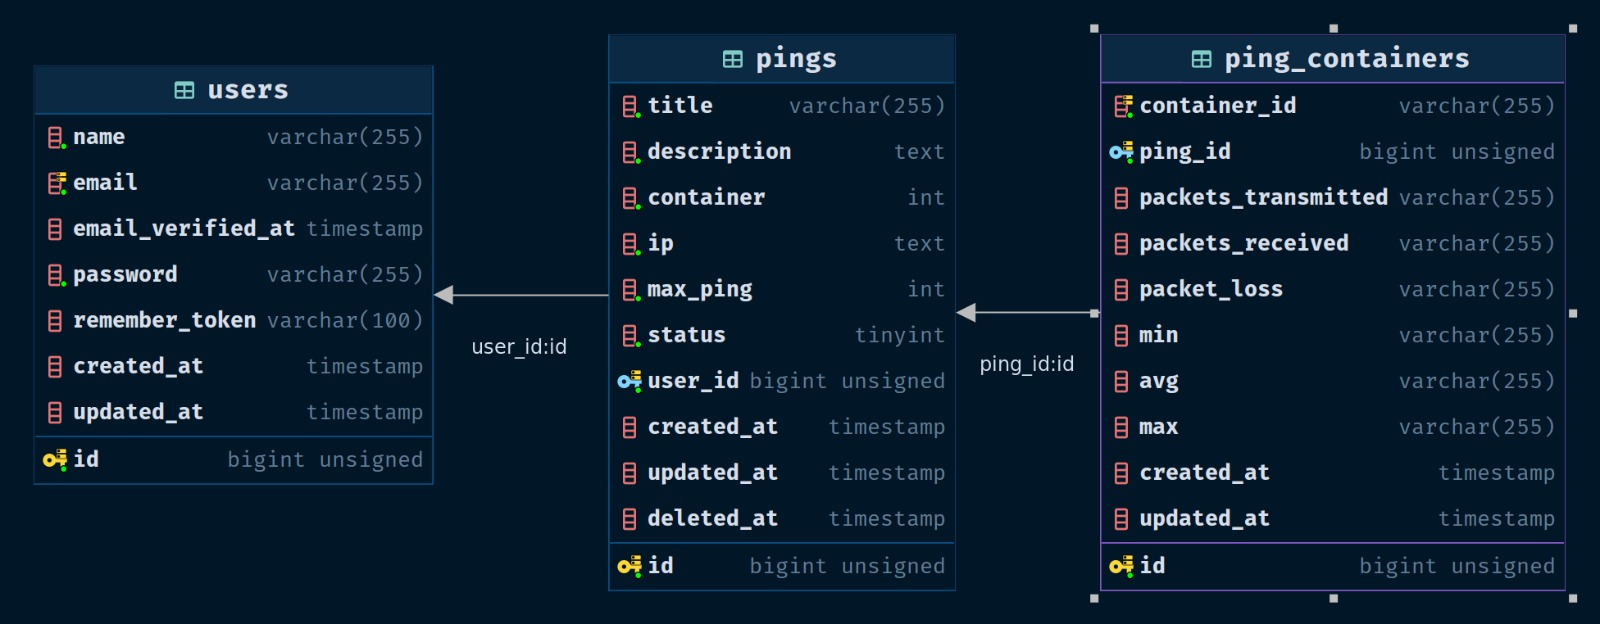
\includegraphics[width=0.9\textwidth]{sql.jpg}
    \caption{Sql ping tabloları}
    \label{fig:resim_etiketi}
  \end{figure}


